\section{Research}

\subsection{June 16 New Cone Definition for Dyadic Cubes}
\begin{definition}[Dyadic Cubes]
    $[m 2^{-k}, (m+1)2^{-k}) \times [l2^{-k}, (l+1)2^{-k})$, $m,l\in\ZZ$
\end{definition}

\begin{definition}[Bad Cone at a Cube(definition 1)] Let $Q$ be the dyadic cube, then we can have the first definition of bad cone at $Q$ with respect to $V$ and $\alpha$ by:
    $$C^1_{\mathcal{B}}(Q, V, \alpha) := \bigcup_{x\in Q} C_\mathcal{B}(x, V_x, \alpha)$$
    where $V = \bigcup_x V_x$ where $\{V_x\}$ is a set of m-dimensional linear plane through $x$(i.e. $x\in V_x$) such that $V_x\cap Q\neq\emptyset, Q\subset \{V_x\}$ and any of two distinct planes in the set are parallel with each other. Correspondingly, we also have
    $$
    C^1_{\mathcal{B}}(Q, r, V, \alpha) = C^1_{\mathcal{B}}(Q, V, \alpha) \cap B(x,r)
    $$
\end{definition}

\begin{definition}[Bad Cone for Cube(definition 2)]
    We can have the second definition of bad cone at $Q$ with respect to $V$ and $\alpha$ with the similar notation:
    $$C^2_{\mathcal{B}}(Q, V, \alpha) := \bigcap_{x\in Q} C_\mathcal{B}(x, V_x, \alpha), \quad
    C^2_{\mathcal{B}}(Q, r, V, \alpha) = C^2_{\mathcal{B}}(Q, V, \alpha) \cap B(x,r)
    $$
\end{definition}
\begin{figure}[H]
    \centering
    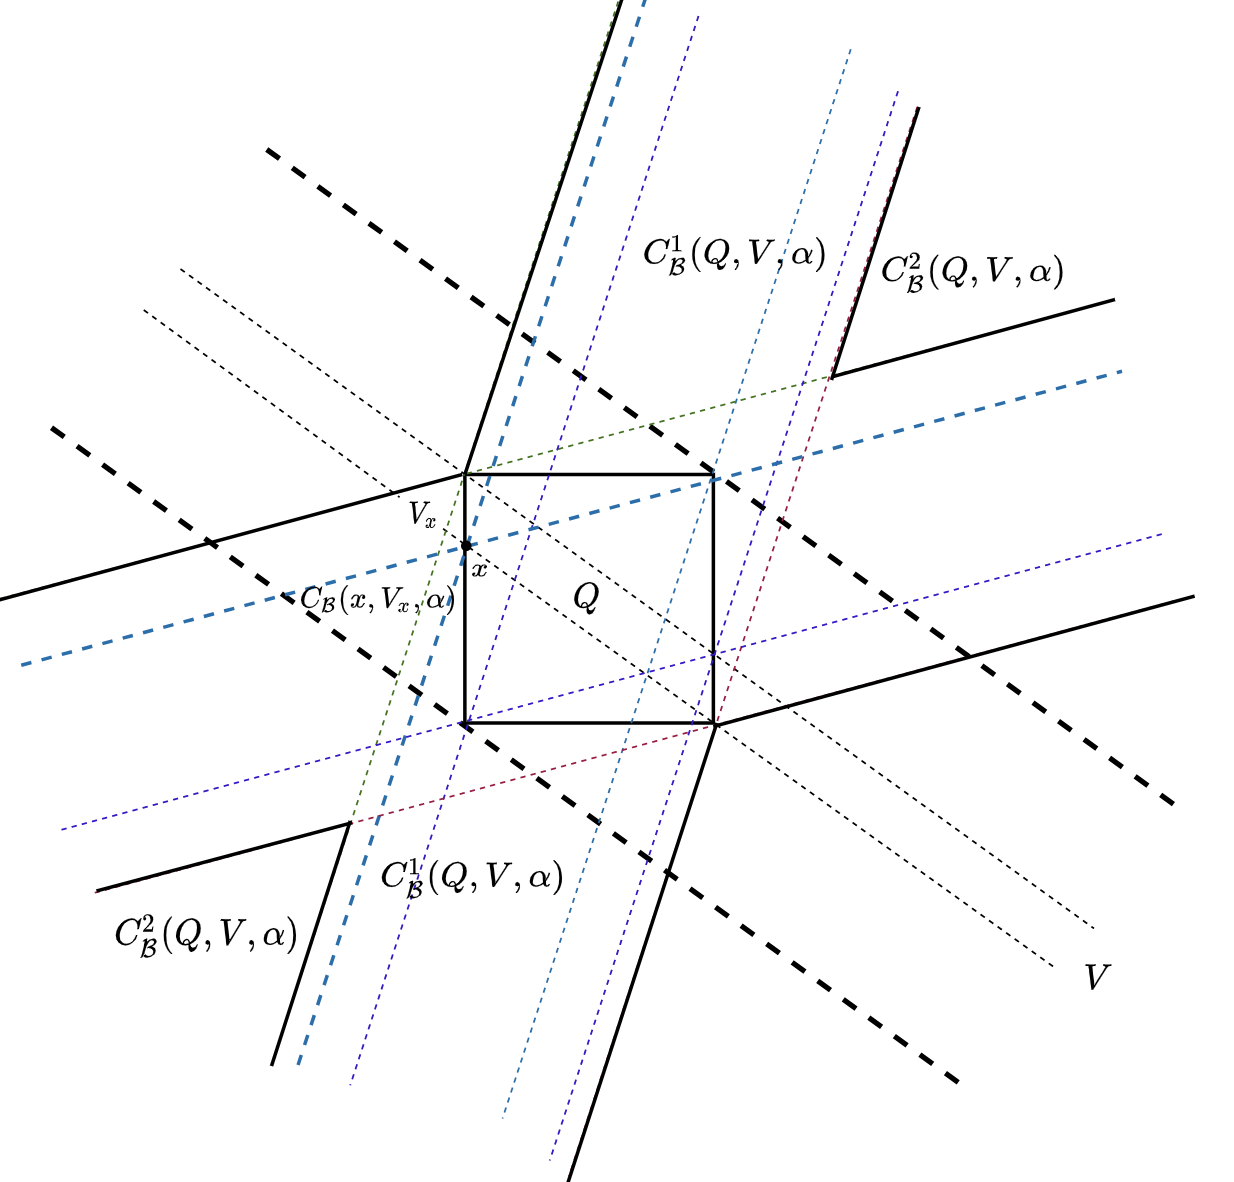
\includegraphics[width=.66\textwidth]{images/cubebadconeDef.png}
    \caption{Visulize two definitions of bad cone at a cube in $\RR^2$}
\end{figure}

\begin{problem}
    Suppose that at $\mu$-a.e. $x$, for all $k$, the cube of side length $2^{-k}$ containing $x$ satisfies
    $$
    \mu(C^2_\mathcal{B}(Q, r, V, \alpha)) = 0
    $$
    is $\mu$-carried Lipschitz by Lipschitz graphs?
\end{problem}

\newpage
\subsection{June 15 A Proposition of Doubling Measure for Cubes}

\begin{proposition}
    If $\forall x\in \RR^2, \mu(B(x, 2r))\leq K\mu(B(x,r)), K\in\ZZ^+$, then $\exists R\in \ZZ^+$ s.t. $\mu(3Q)\leq R\mu(Q)$ where $Q$ is the cube, 3$Q$ is the cube with triple side length with same center as $Q$. 
\end{proposition}
\proof  $\mu(3Q) \leq \mu(B(x, 4r)) \leq K^2\mu(B(x, r))\leq K^2 \mu(Q)$ due to doubling measure and containment. 

\begin{figure}[H]
    \centering
    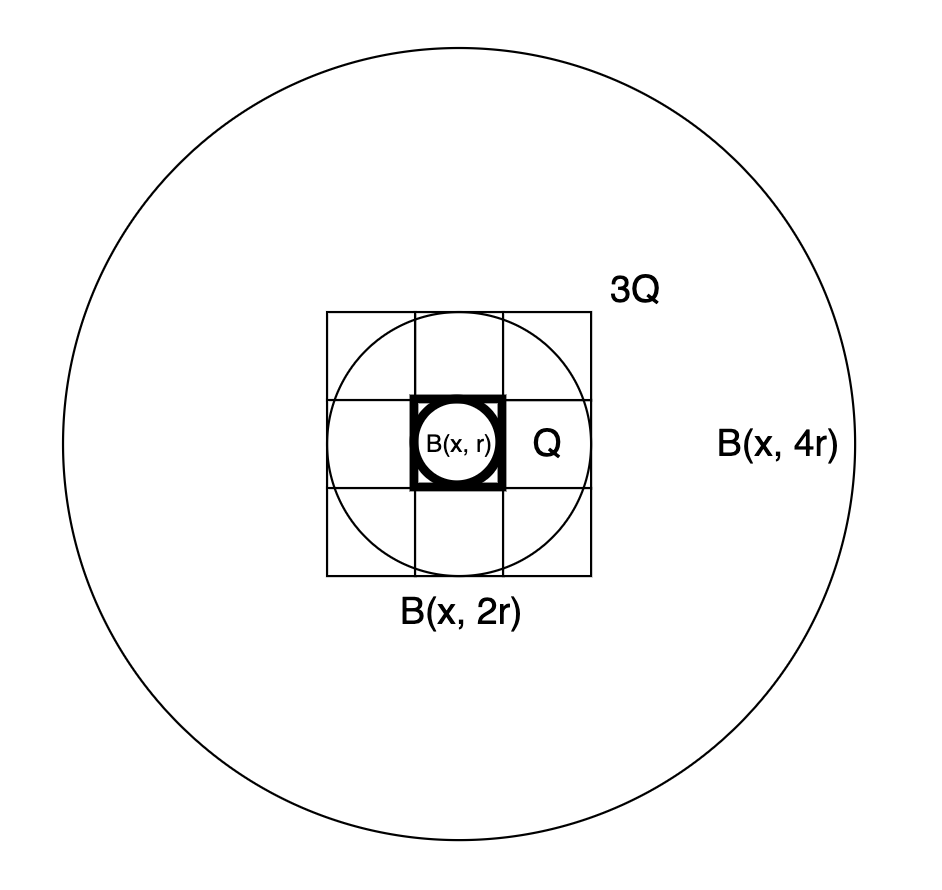
\includegraphics[width=.66\textwidth]{images/doubleMcube.png}
\end{figure}


\newpage
\subsection{June 14 Paper \texorpdfstring{\cite{naples2020}}{Lg} Sec. 7 Graph Rectifiable Measures}
